\documentclass[11pt]{article}
\usepackage[textwidth=18.0cm, textheight=23.0cm, top=2.0cm]{geometry}
\usepackage{pst-all}
\usepackage{amssymb}
\usepackage{tikz}
\usepackage{underscore}\begin{document}
\pagestyle{empty}


ClassName: \underline{\textbf{Class_08.2bp-23}}
\par
BinSize: \underline{\textbf{100 × 100}}
\par
ReduceSize: \underline{\textbf{100 × 100}}
\par
TypeNum: \underline{\textbf{60}}
\par
Num: \underline{\textbf{60}}
\par
OutS: \underline{\textbf{150000}}
\par
InS: \underline{\textbf{124539}}
\par
Rate: \underline{\textbf{0.830}}
\par
UB: \underline{\textbf{15}}
\par
LB0: \underline{\textbf{15}}
\par
LB: \underline{\textbf{15}}
\par
LBWithCut: \underline{\textbf{15}}
\par
NodeCut: \underline{\textbf{0}}
\par
ExtendedNodeCnt: \underline{\textbf{1}}
\par
GenNodeCnt: \underline{\textbf{1}}
\par
PrimalNode: \underline{\textbf{0}}
\par
ColumnCount: \underline{\textbf{15}}
\par
TotalCutCount: \underline{\textbf{0}}
\par
RootCutCount: \underline{\textbf{0}}
\par
LPSolverCnt: \underline{\textbf{1}}
\par
PricingSolverCnt: \underline{\textbf{0}}
\par
BranchAndBoundNum: \underline{\textbf{1}}
\par
isOpt: \underline{\textbf{true}}
\par
TimeOnInitSolution: \underline{\textbf{600.000 s}}
\par
TimeOnPrimal: \underline{\textbf{0.000 s}}
\par
TimeOnPricing: \underline{\textbf{0.000 s}}
\par
TimeOnRmp: \underline{\textbf{0.078 s}}
\par
TotalTime: \underline{\textbf{600.375 s}}
\par
\newpage


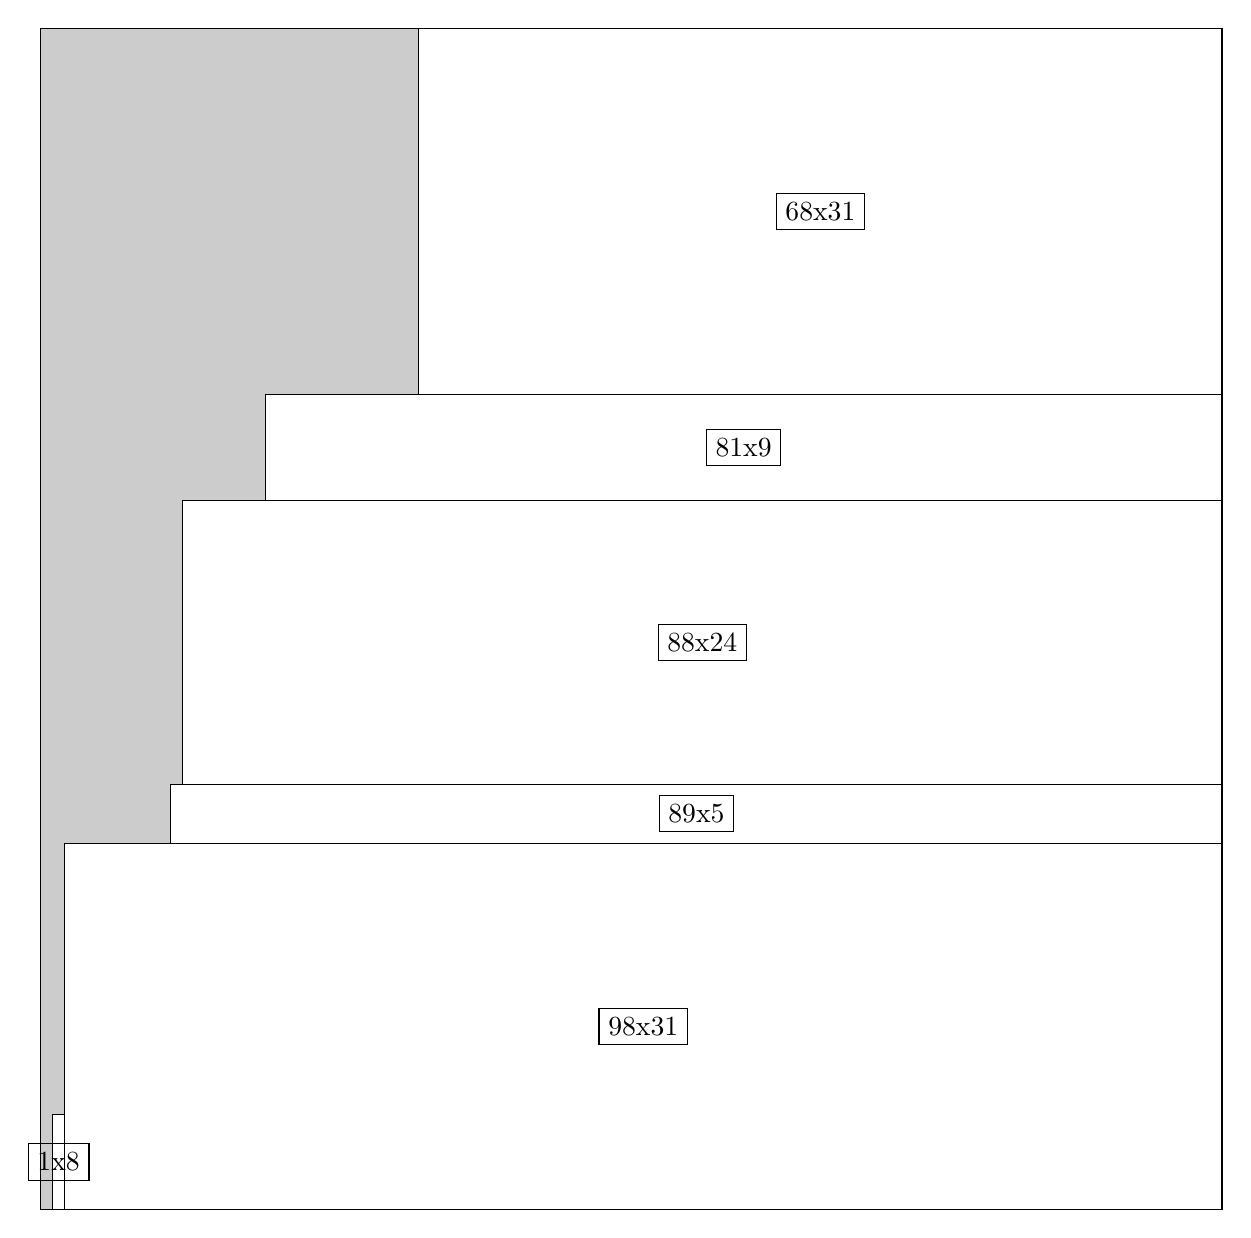
\begin{tikzpicture}[shorten >=1pt,scale=1.0,every node/.style={scale=1.0},->]
\tikzstyle{vertex}=[circle,fill=black!25,minimum size=14pt,inner sep=0pt]
\filldraw[fill=gray!40!white, draw=black] (0,0) rectangle (15.0,15.0);
\foreach \name/\x/\y/\w/\h in {98x31/0.3/0.0/14.7/4.6499999999999995,1x8/0.15/0.0/0.15/1.2,89x5/1.65/4.6499999999999995/13.35/0.75,88x24/1.7999999999999998/5.3999999999999995/13.2/3.5999999999999996,81x9/2.85/9.0/12.15/1.3499999999999999,68x31/4.8/10.35/10.2/4.6499999999999995}
\filldraw[fill=white!40!white, draw=black] (\x,\y) rectangle node[draw] (\name) {\name} ++(\w,\h);
\end{tikzpicture}


w =98 , h =31 , x =2 , y =0 , v =3038
\par
w =1 , h =8 , x =1 , y =0 , v =8
\par
w =89 , h =5 , x =11 , y =31 , v =445
\par
w =88 , h =24 , x =12 , y =36 , v =2112
\par
w =81 , h =9 , x =19 , y =60 , v =729
\par
w =68 , h =31 , x =32 , y =69 , v =2108
\par
\newpage


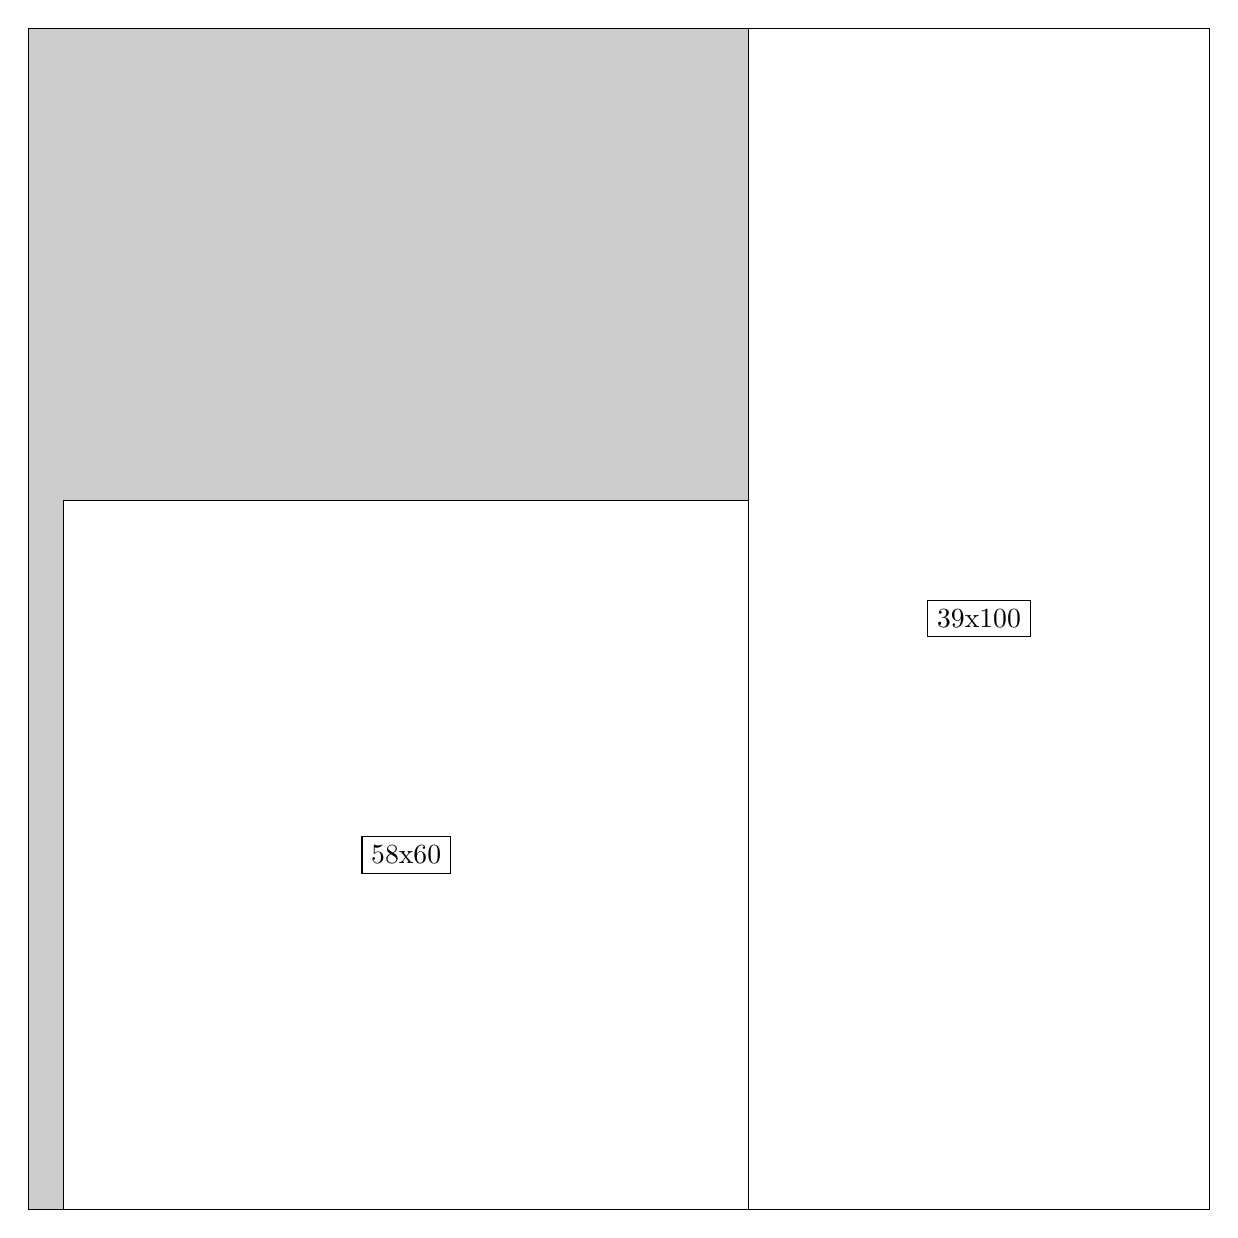
\begin{tikzpicture}[shorten >=1pt,scale=1.0,every node/.style={scale=1.0},->]
\tikzstyle{vertex}=[circle,fill=black!25,minimum size=14pt,inner sep=0pt]
\filldraw[fill=gray!40!white, draw=black] (0,0) rectangle (15.0,15.0);
\foreach \name/\x/\y/\w/\h in {39x100/9.15/0.0/5.85/15.0,58x60/0.44999999999999996/0.0/8.7/9.0}
\filldraw[fill=white!40!white, draw=black] (\x,\y) rectangle node[draw] (\name) {\name} ++(\w,\h);
\end{tikzpicture}


w =39 , h =100 , x =61 , y =0 , v =3900
\par
w =58 , h =60 , x =3 , y =0 , v =3480
\par
\newpage


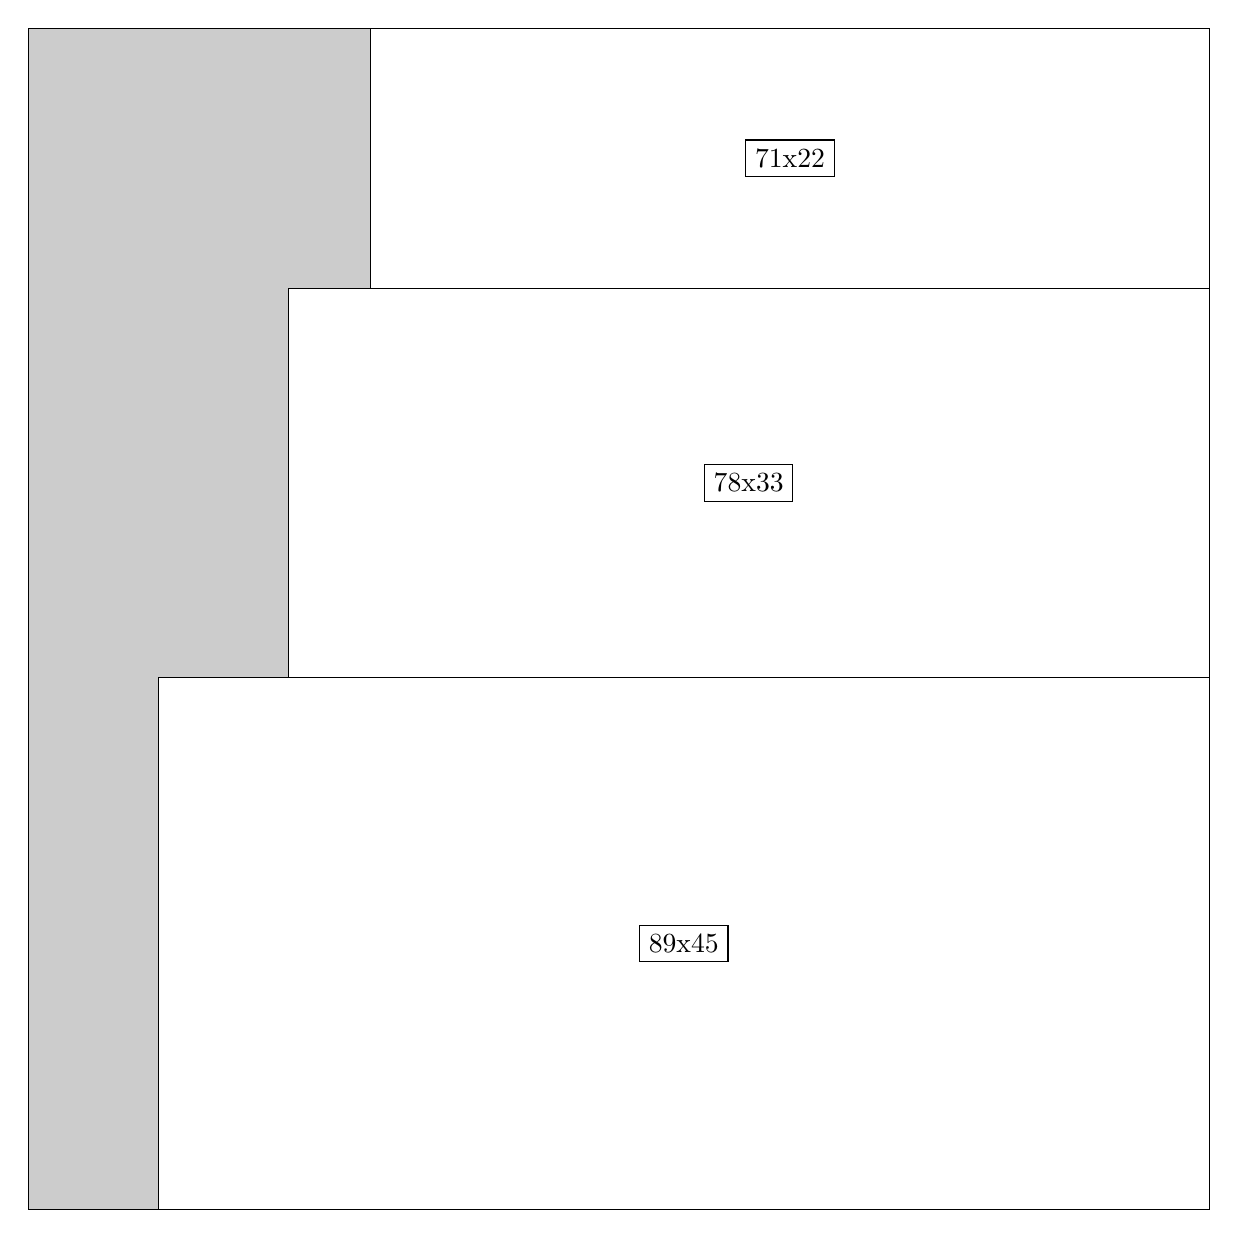
\begin{tikzpicture}[shorten >=1pt,scale=1.0,every node/.style={scale=1.0},->]
\tikzstyle{vertex}=[circle,fill=black!25,minimum size=14pt,inner sep=0pt]
\filldraw[fill=gray!40!white, draw=black] (0,0) rectangle (15.0,15.0);
\foreach \name/\x/\y/\w/\h in {89x45/1.65/0.0/13.35/6.75,78x33/3.3/6.75/11.7/4.95,71x22/4.35/11.7/10.65/3.3}
\filldraw[fill=white!40!white, draw=black] (\x,\y) rectangle node[draw] (\name) {\name} ++(\w,\h);
\end{tikzpicture}


w =89 , h =45 , x =11 , y =0 , v =4005
\par
w =78 , h =33 , x =22 , y =45 , v =2574
\par
w =71 , h =22 , x =29 , y =78 , v =1562
\par
\newpage


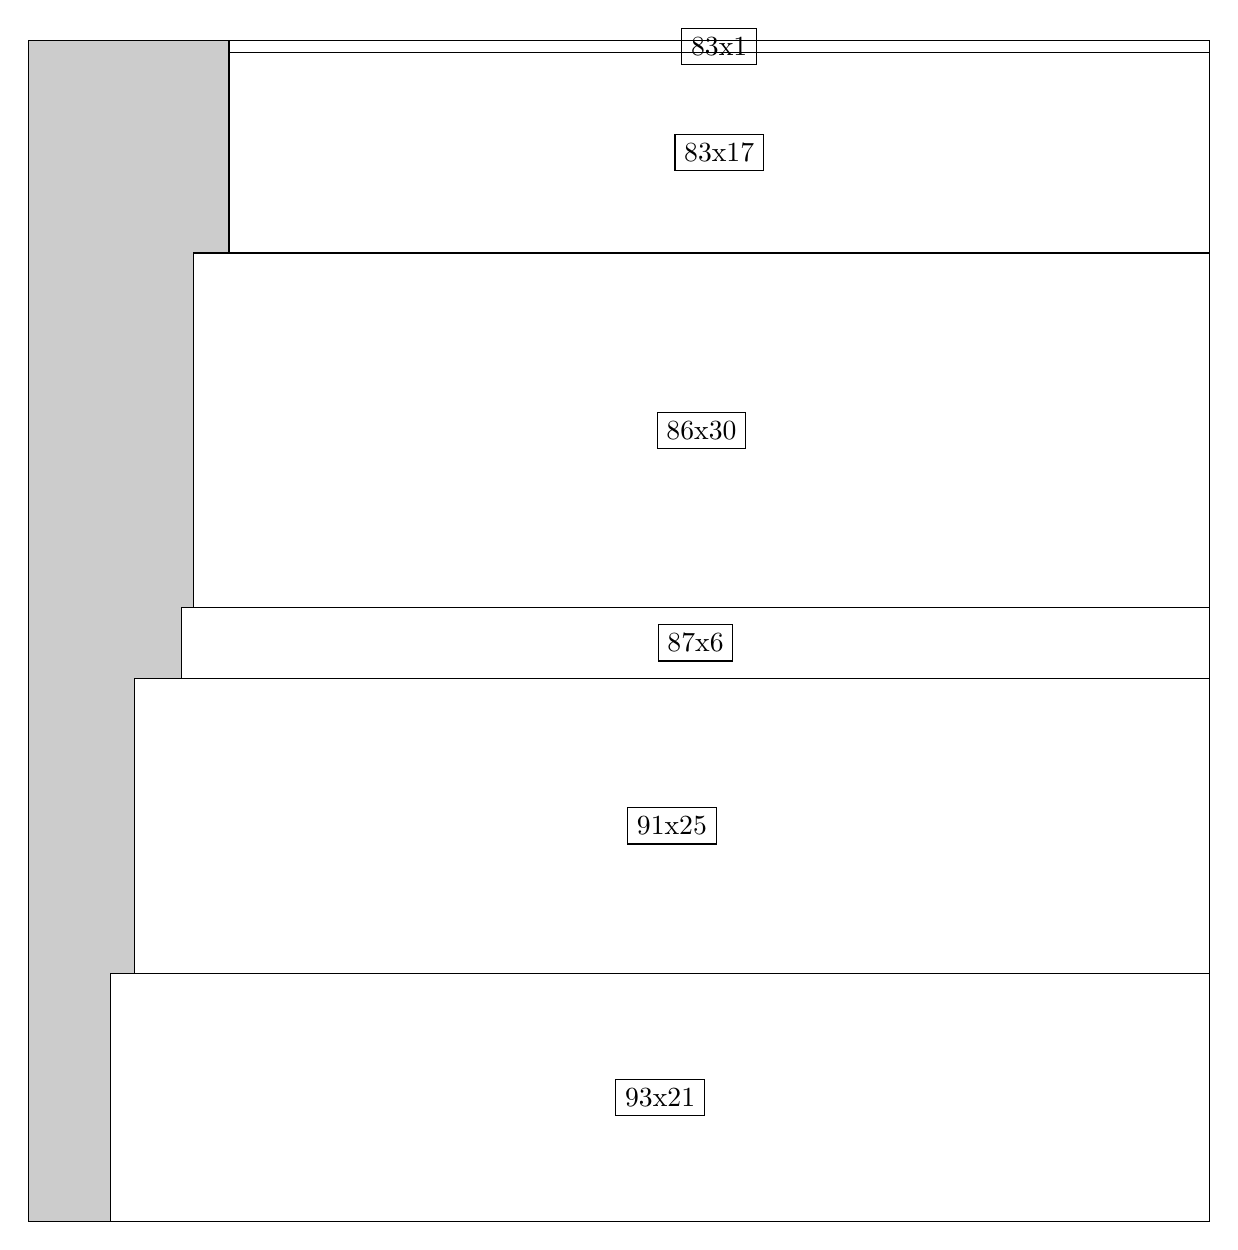
\begin{tikzpicture}[shorten >=1pt,scale=1.0,every node/.style={scale=1.0},->]
\tikzstyle{vertex}=[circle,fill=black!25,minimum size=14pt,inner sep=0pt]
\filldraw[fill=gray!40!white, draw=black] (0,0) rectangle (15.0,15.0);
\foreach \name/\x/\y/\w/\h in {93x21/1.05/0.0/13.95/3.15,91x25/1.3499999999999999/3.15/13.65/3.75,87x6/1.95/6.8999999999999995/13.049999999999999/0.8999999999999999,86x30/2.1/7.8/12.9/4.5,83x17/2.55/12.299999999999999/12.45/2.55,83x1/2.55/14.85/12.45/0.15}
\filldraw[fill=white!40!white, draw=black] (\x,\y) rectangle node[draw] (\name) {\name} ++(\w,\h);
\end{tikzpicture}


w =93 , h =21 , x =7 , y =0 , v =1953
\par
w =91 , h =25 , x =9 , y =21 , v =2275
\par
w =87 , h =6 , x =13 , y =46 , v =522
\par
w =86 , h =30 , x =14 , y =52 , v =2580
\par
w =83 , h =17 , x =17 , y =82 , v =1411
\par
w =83 , h =1 , x =17 , y =99 , v =83
\par
\newpage


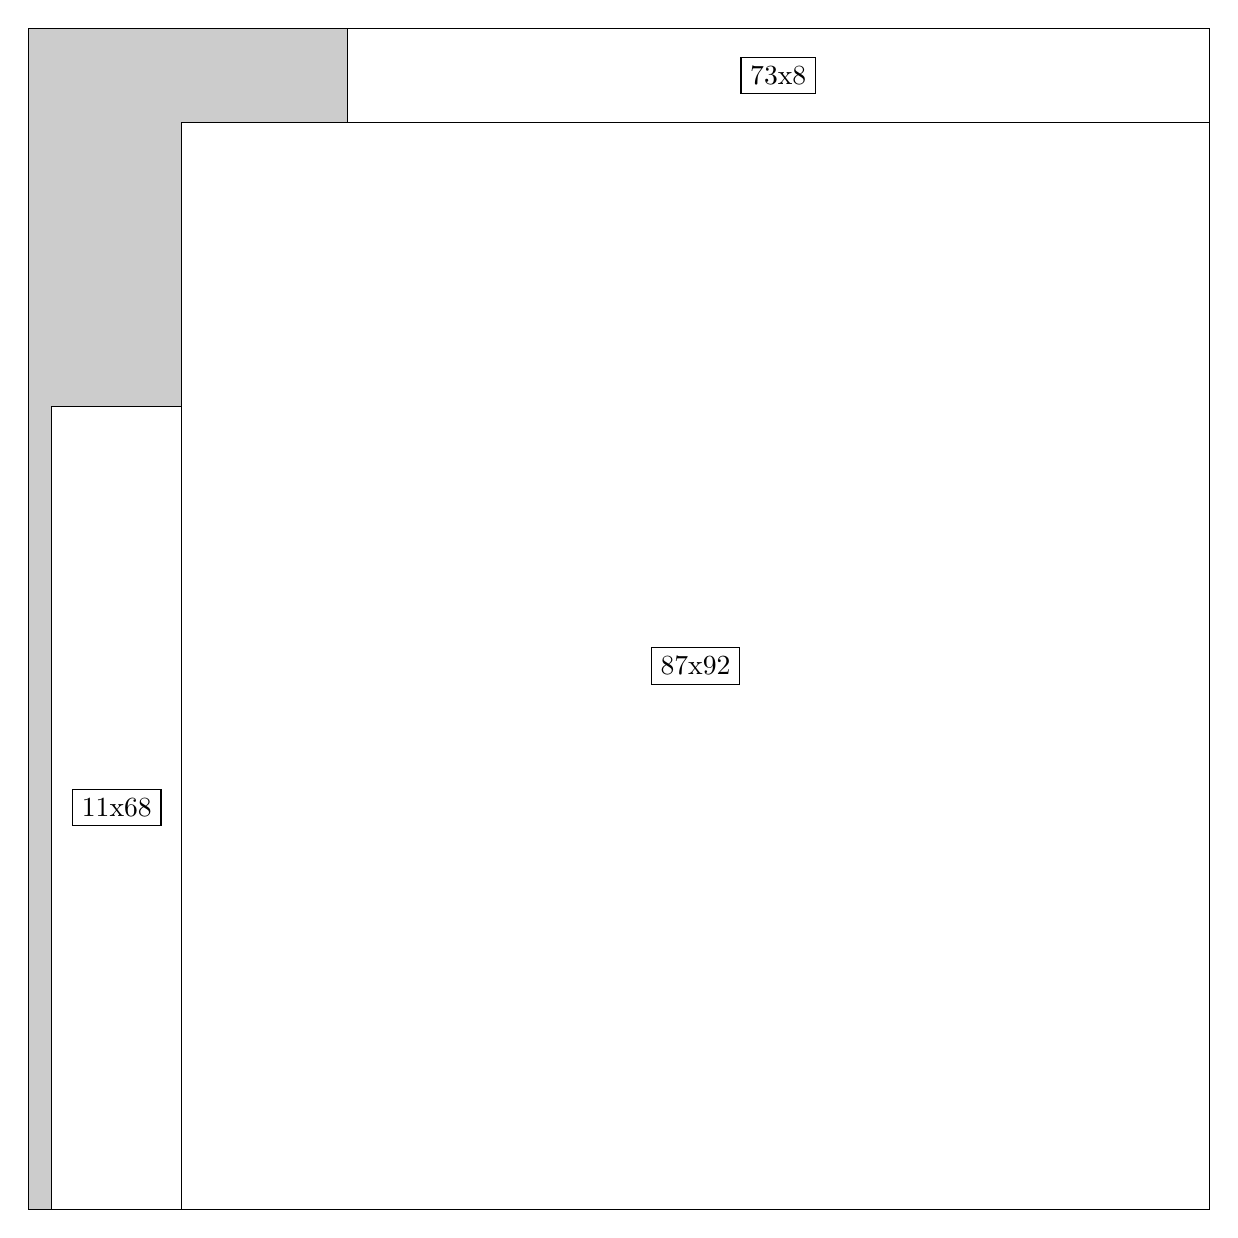
\begin{tikzpicture}[shorten >=1pt,scale=1.0,every node/.style={scale=1.0},->]
\tikzstyle{vertex}=[circle,fill=black!25,minimum size=14pt,inner sep=0pt]
\filldraw[fill=gray!40!white, draw=black] (0,0) rectangle (15.0,15.0);
\foreach \name/\x/\y/\w/\h in {87x92/1.95/0.0/13.049999999999999/13.799999999999999,11x68/0.3/0.0/1.65/10.2,73x8/4.05/13.799999999999999/10.95/1.2}
\filldraw[fill=white!40!white, draw=black] (\x,\y) rectangle node[draw] (\name) {\name} ++(\w,\h);
\end{tikzpicture}


w =87 , h =92 , x =13 , y =0 , v =8004
\par
w =11 , h =68 , x =2 , y =0 , v =748
\par
w =73 , h =8 , x =27 , y =92 , v =584
\par
\newpage


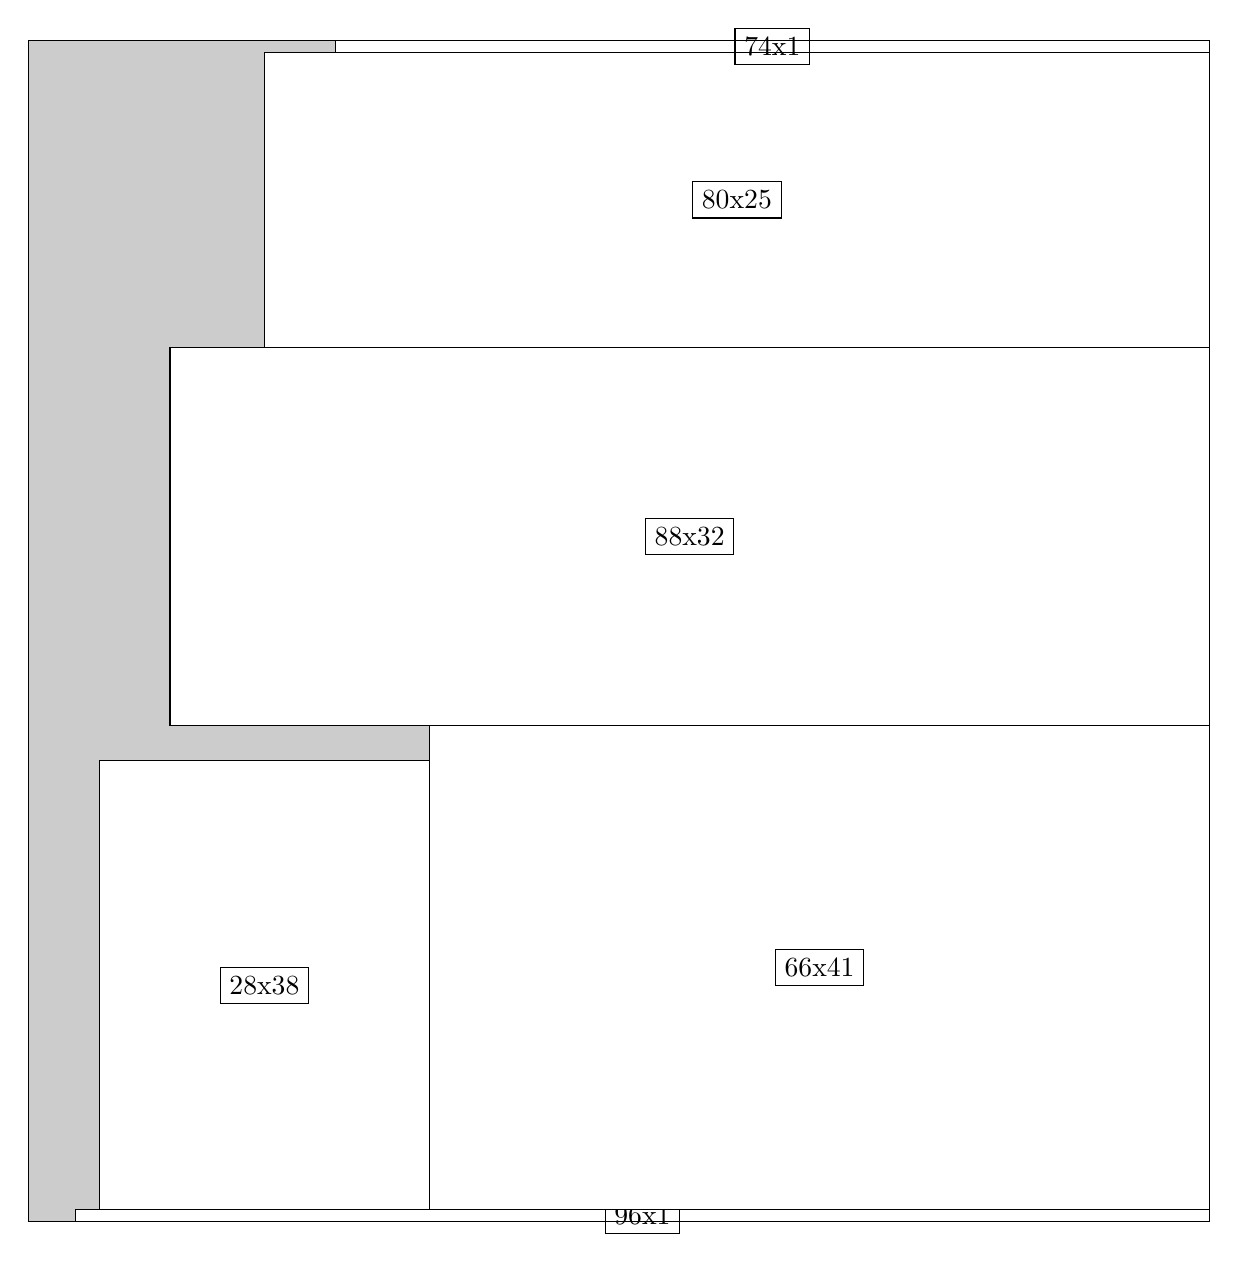
\begin{tikzpicture}[shorten >=1pt,scale=1.0,every node/.style={scale=1.0},->]
\tikzstyle{vertex}=[circle,fill=black!25,minimum size=14pt,inner sep=0pt]
\filldraw[fill=gray!40!white, draw=black] (0,0) rectangle (15.0,15.0);
\foreach \name/\x/\y/\w/\h in {96x1/0.6/0.0/14.399999999999999/0.15,66x41/5.1/0.15/9.9/6.1499999999999995,28x38/0.8999999999999999/0.15/4.2/5.7,88x32/1.7999999999999998/6.3/13.2/4.8,80x25/3.0/11.1/12.0/3.75,74x1/3.9/14.85/11.1/0.15}
\filldraw[fill=white!40!white, draw=black] (\x,\y) rectangle node[draw] (\name) {\name} ++(\w,\h);
\end{tikzpicture}


w =96 , h =1 , x =4 , y =0 , v =96
\par
w =66 , h =41 , x =34 , y =1 , v =2706
\par
w =28 , h =38 , x =6 , y =1 , v =1064
\par
w =88 , h =32 , x =12 , y =42 , v =2816
\par
w =80 , h =25 , x =20 , y =74 , v =2000
\par
w =74 , h =1 , x =26 , y =99 , v =74
\par
\newpage



\begin{tikzpicture}[shorten >=1pt,scale=1.0,every node/.style={scale=1.0},->]
\tikzstyle{vertex}=[circle,fill=black!25,minimum size=14pt,inner sep=0pt]
\filldraw[fill=gray!40!white, draw=black] (0,0) rectangle (15.0,15.0);
\foreach \name/\x/\y/\w/\h in {65x99/5.25/0.0/9.75/14.85}
\filldraw[fill=white!40!white, draw=black] (\x,\y) rectangle node[draw] (\name) {\name} ++(\w,\h);
\end{tikzpicture}


w =65 , h =99 , x =35 , y =0 , v =6435
\par
\newpage


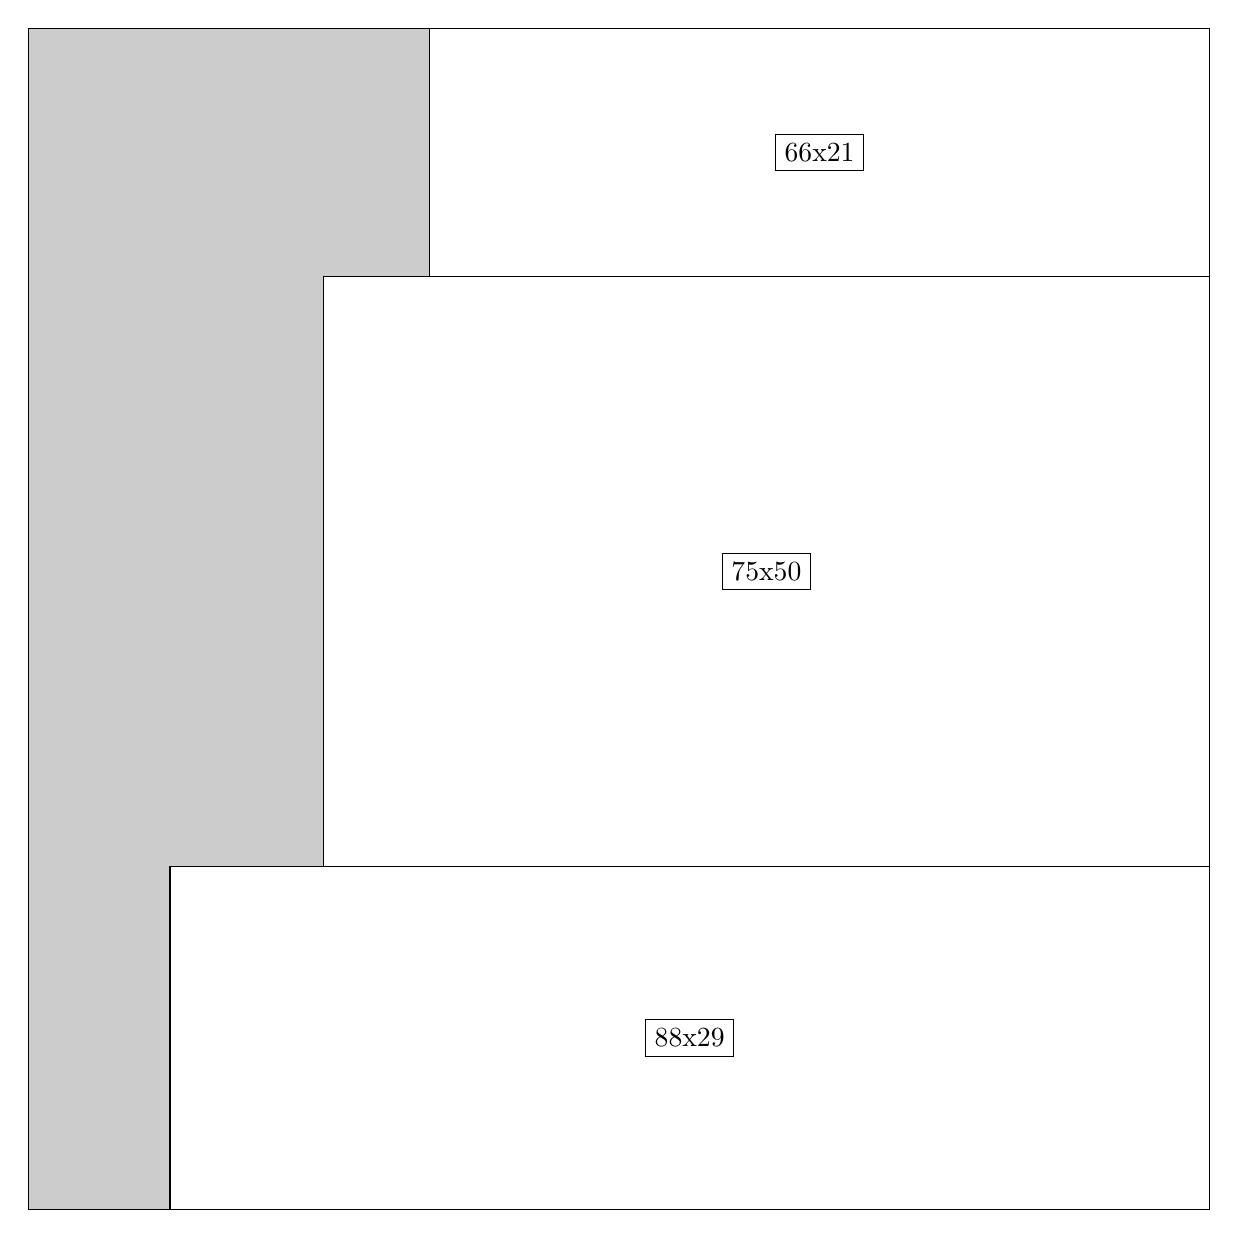
\begin{tikzpicture}[shorten >=1pt,scale=1.0,every node/.style={scale=1.0},->]
\tikzstyle{vertex}=[circle,fill=black!25,minimum size=14pt,inner sep=0pt]
\filldraw[fill=gray!40!white, draw=black] (0,0) rectangle (15.0,15.0);
\foreach \name/\x/\y/\w/\h in {88x29/1.7999999999999998/0.0/13.2/4.35,75x50/3.75/4.35/11.25/7.5,66x21/5.1/11.85/9.9/3.15}
\filldraw[fill=white!40!white, draw=black] (\x,\y) rectangle node[draw] (\name) {\name} ++(\w,\h);
\end{tikzpicture}


w =88 , h =29 , x =12 , y =0 , v =2552
\par
w =75 , h =50 , x =25 , y =29 , v =3750
\par
w =66 , h =21 , x =34 , y =79 , v =1386
\par
\newpage


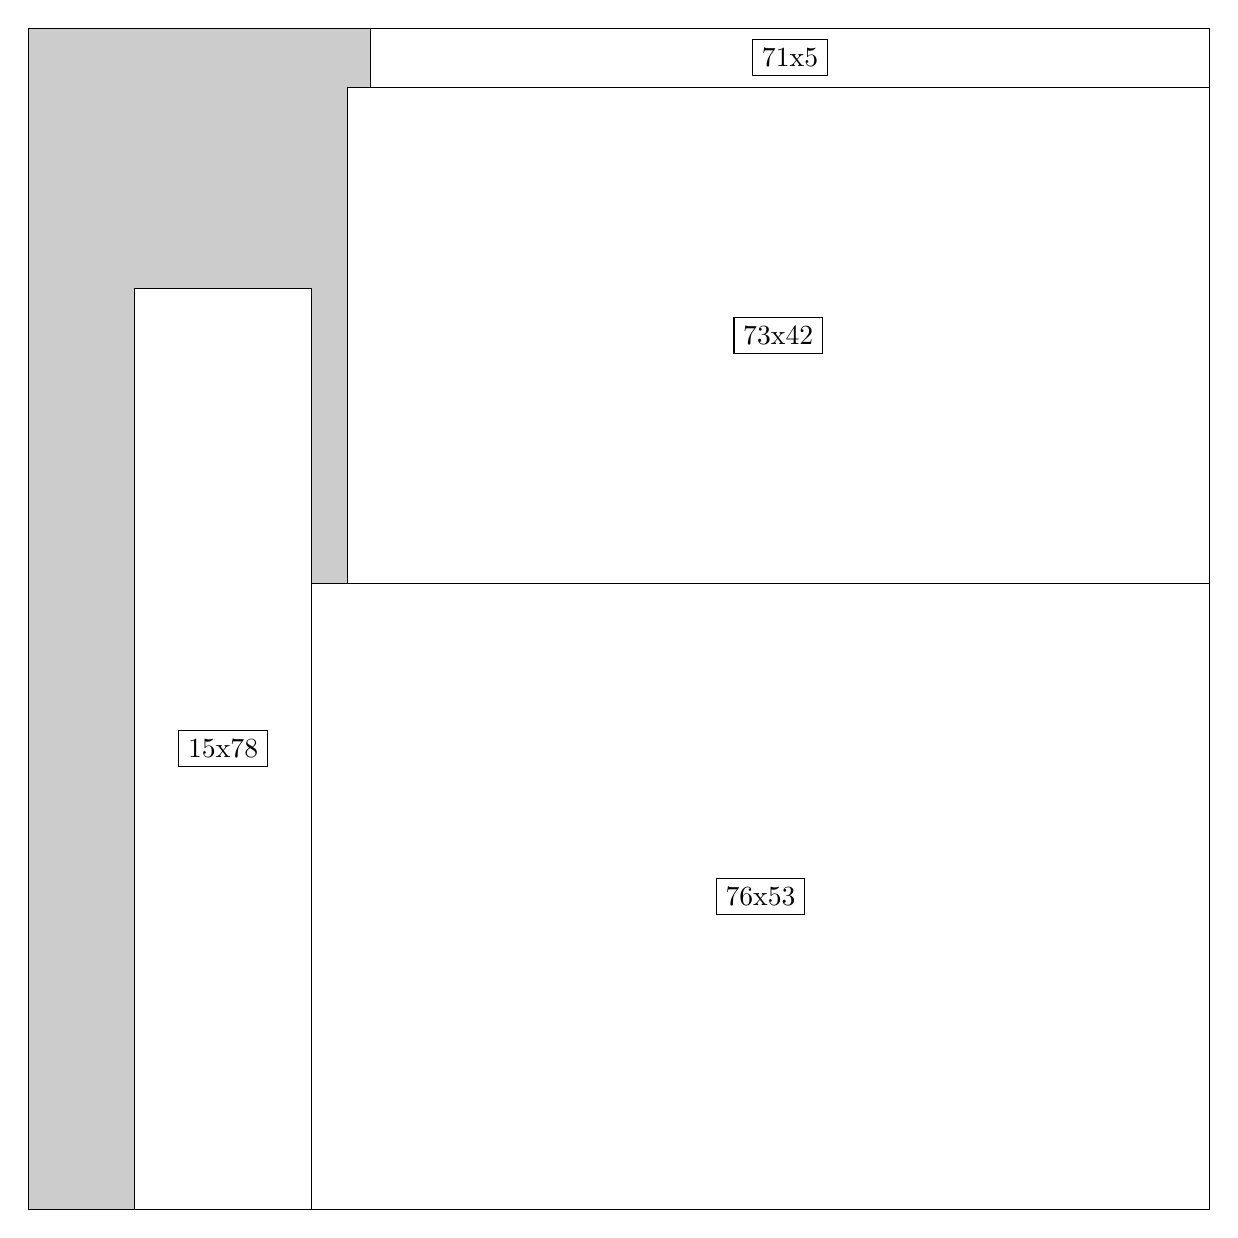
\begin{tikzpicture}[shorten >=1pt,scale=1.0,every node/.style={scale=1.0},->]
\tikzstyle{vertex}=[circle,fill=black!25,minimum size=14pt,inner sep=0pt]
\filldraw[fill=gray!40!white, draw=black] (0,0) rectangle (15.0,15.0);
\foreach \name/\x/\y/\w/\h in {76x53/3.5999999999999996/0.0/11.4/7.949999999999999,73x42/4.05/7.949999999999999/10.95/6.3,71x5/4.35/14.25/10.65/0.75,15x78/1.3499999999999999/0.0/2.25/11.7}
\filldraw[fill=white!40!white, draw=black] (\x,\y) rectangle node[draw] (\name) {\name} ++(\w,\h);
\end{tikzpicture}


w =76 , h =53 , x =24 , y =0 , v =4028
\par
w =73 , h =42 , x =27 , y =53 , v =3066
\par
w =71 , h =5 , x =29 , y =95 , v =355
\par
w =15 , h =78 , x =9 , y =0 , v =1170
\par
\newpage


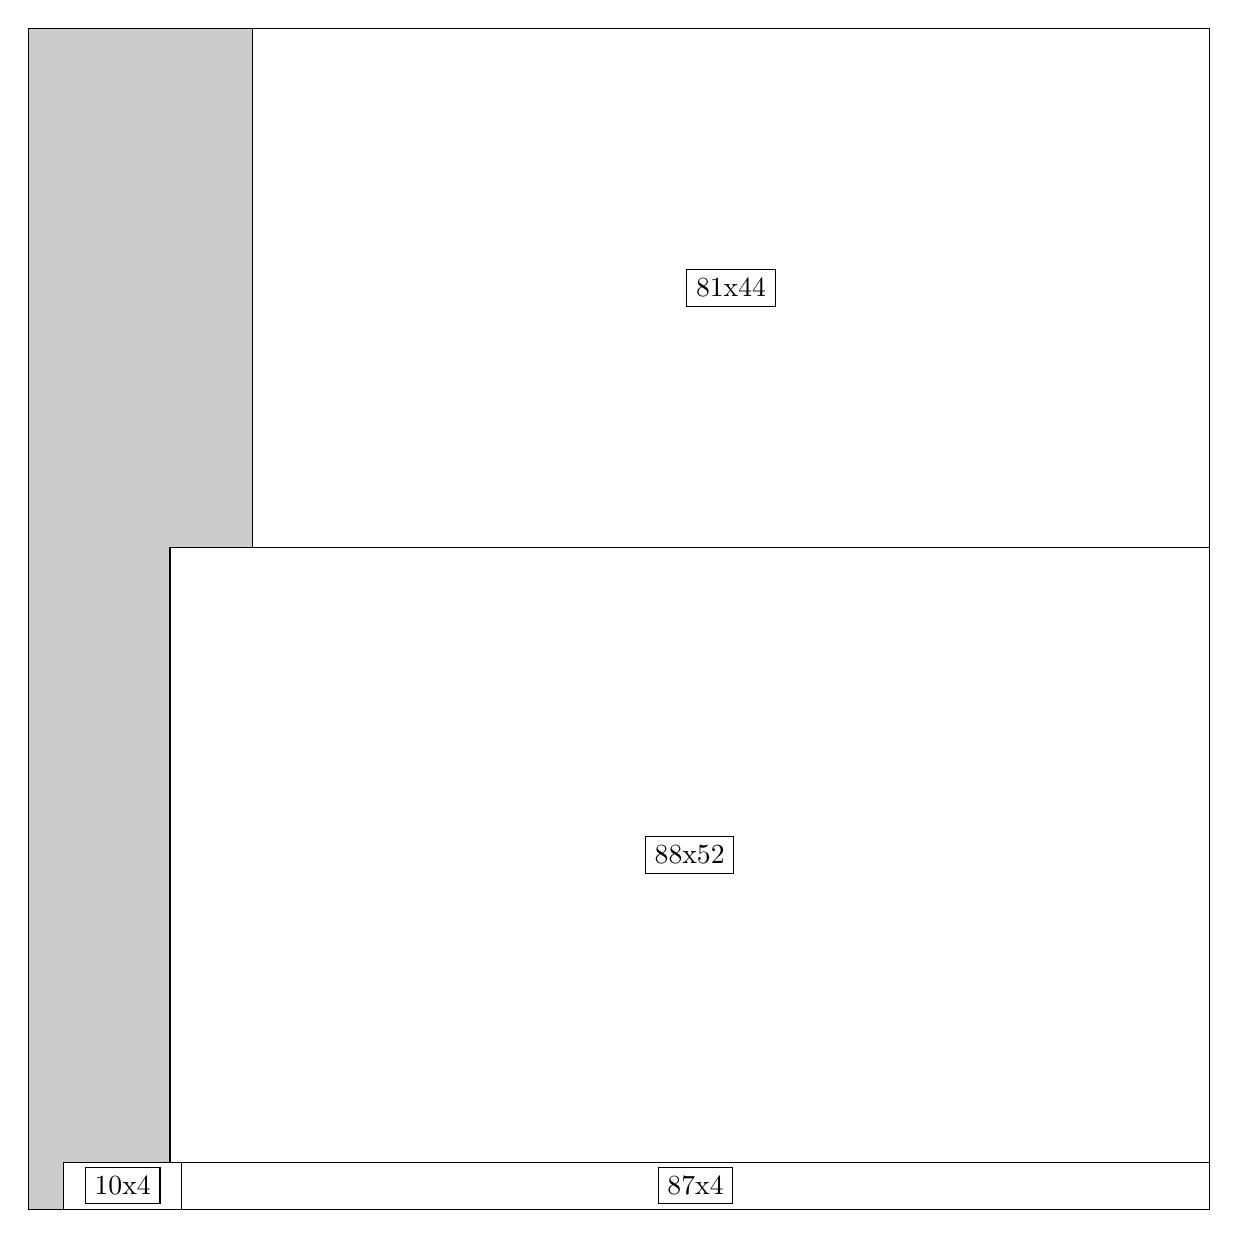
\begin{tikzpicture}[shorten >=1pt,scale=1.0,every node/.style={scale=1.0},->]
\tikzstyle{vertex}=[circle,fill=black!25,minimum size=14pt,inner sep=0pt]
\filldraw[fill=gray!40!white, draw=black] (0,0) rectangle (15.0,15.0);
\foreach \name/\x/\y/\w/\h in {87x4/1.95/0.0/13.049999999999999/0.6,10x4/0.44999999999999996/0.0/1.5/0.6,88x52/1.7999999999999998/0.6/13.2/7.8,81x44/2.85/8.4/12.15/6.6}
\filldraw[fill=white!40!white, draw=black] (\x,\y) rectangle node[draw] (\name) {\name} ++(\w,\h);
\end{tikzpicture}


w =87 , h =4 , x =13 , y =0 , v =348
\par
w =10 , h =4 , x =3 , y =0 , v =40
\par
w =88 , h =52 , x =12 , y =4 , v =4576
\par
w =81 , h =44 , x =19 , y =56 , v =3564
\par
\newpage


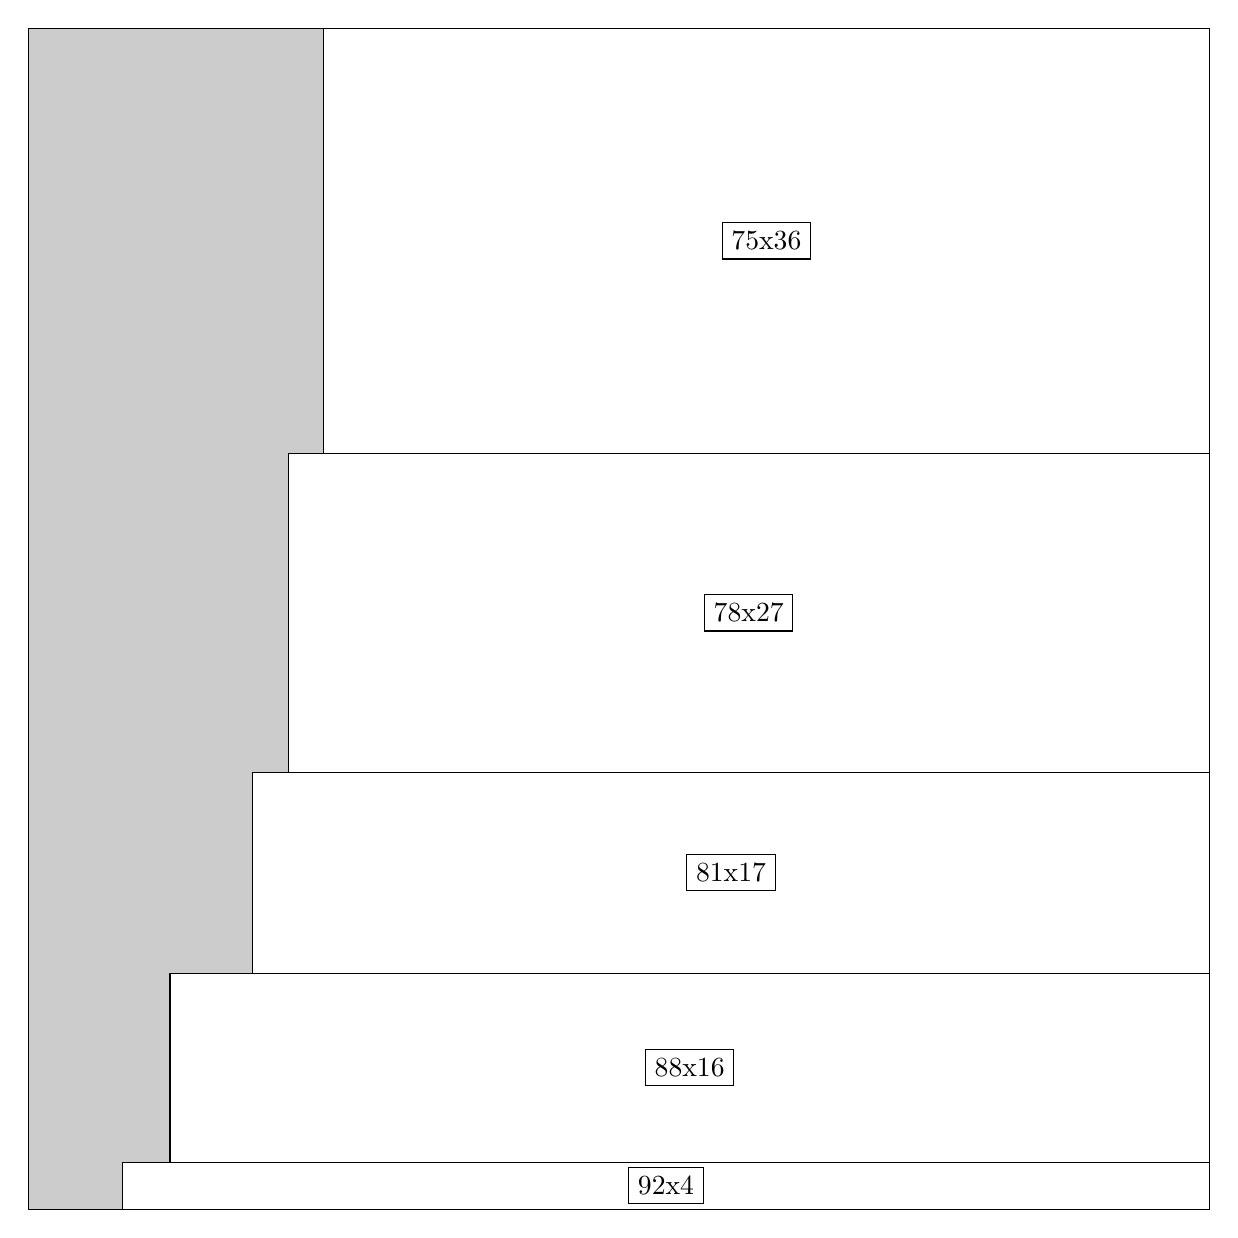
\begin{tikzpicture}[shorten >=1pt,scale=1.0,every node/.style={scale=1.0},->]
\tikzstyle{vertex}=[circle,fill=black!25,minimum size=14pt,inner sep=0pt]
\filldraw[fill=gray!40!white, draw=black] (0,0) rectangle (15.0,15.0);
\foreach \name/\x/\y/\w/\h in {92x4/1.2/0.0/13.799999999999999/0.6,88x16/1.7999999999999998/0.6/13.2/2.4,81x17/2.85/3.0/12.15/2.55,78x27/3.3/5.55/11.7/4.05,75x36/3.75/9.6/11.25/5.3999999999999995}
\filldraw[fill=white!40!white, draw=black] (\x,\y) rectangle node[draw] (\name) {\name} ++(\w,\h);
\end{tikzpicture}


w =92 , h =4 , x =8 , y =0 , v =368
\par
w =88 , h =16 , x =12 , y =4 , v =1408
\par
w =81 , h =17 , x =19 , y =20 , v =1377
\par
w =78 , h =27 , x =22 , y =37 , v =2106
\par
w =75 , h =36 , x =25 , y =64 , v =2700
\par
\newpage


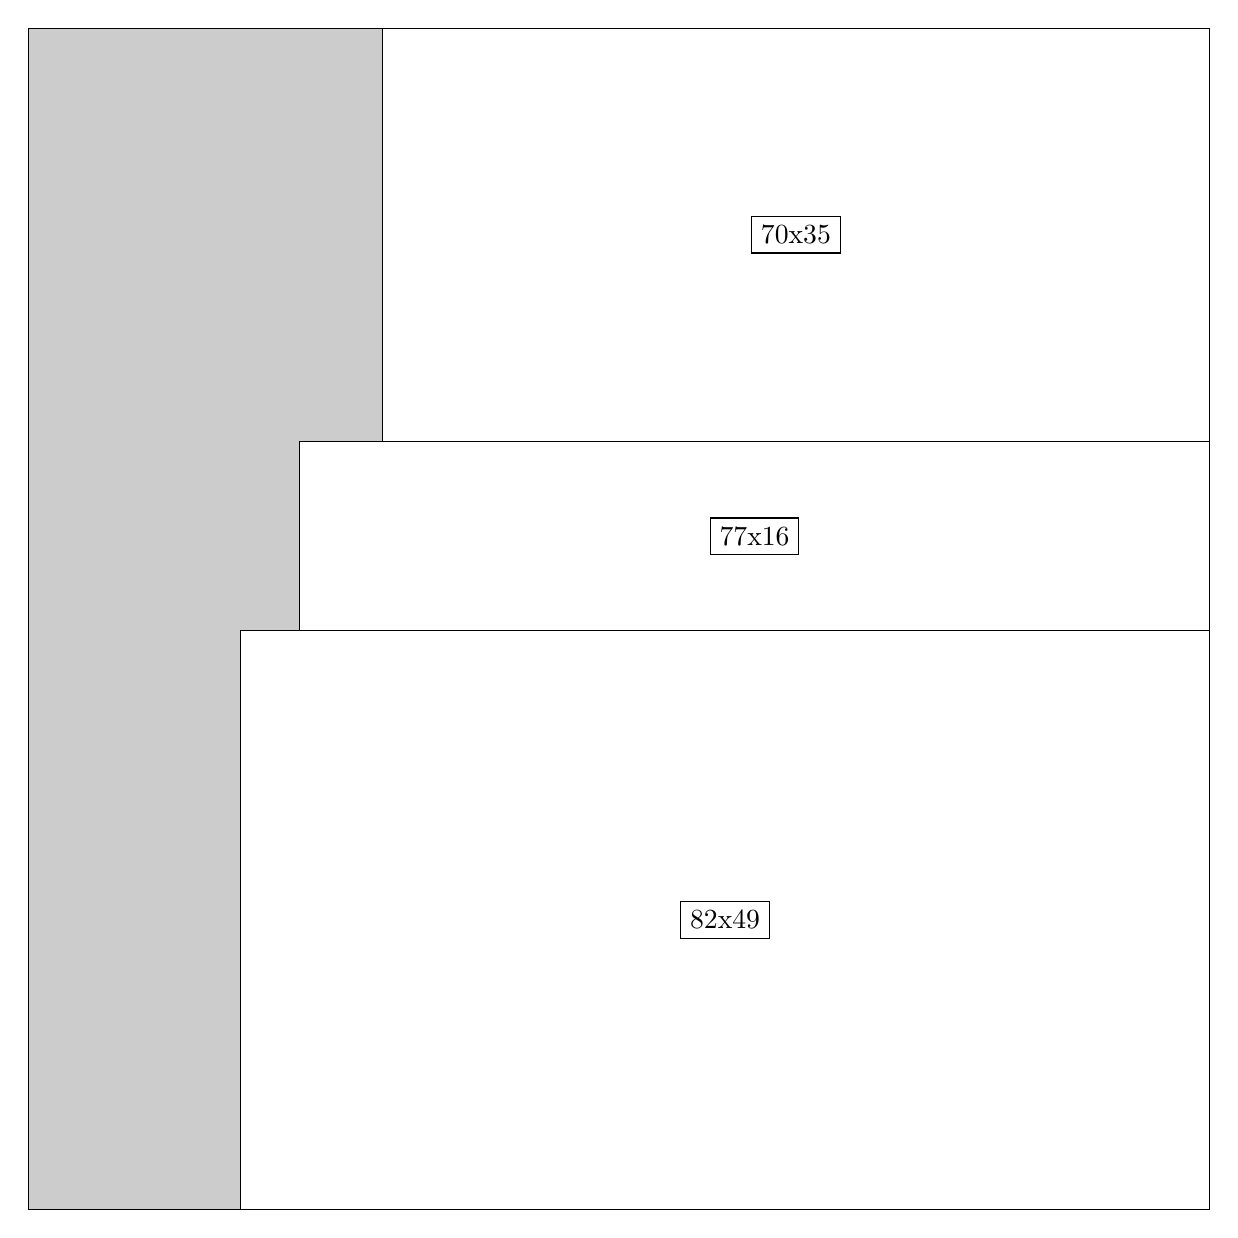
\begin{tikzpicture}[shorten >=1pt,scale=1.0,every node/.style={scale=1.0},->]
\tikzstyle{vertex}=[circle,fill=black!25,minimum size=14pt,inner sep=0pt]
\filldraw[fill=gray!40!white, draw=black] (0,0) rectangle (15.0,15.0);
\foreach \name/\x/\y/\w/\h in {82x49/2.6999999999999997/0.0/12.299999999999999/7.35,77x16/3.4499999999999997/7.35/11.549999999999999/2.4,70x35/4.5/9.75/10.5/5.25}
\filldraw[fill=white!40!white, draw=black] (\x,\y) rectangle node[draw] (\name) {\name} ++(\w,\h);
\end{tikzpicture}


w =82 , h =49 , x =18 , y =0 , v =4018
\par
w =77 , h =16 , x =23 , y =49 , v =1232
\par
w =70 , h =35 , x =30 , y =65 , v =2450
\par
\newpage


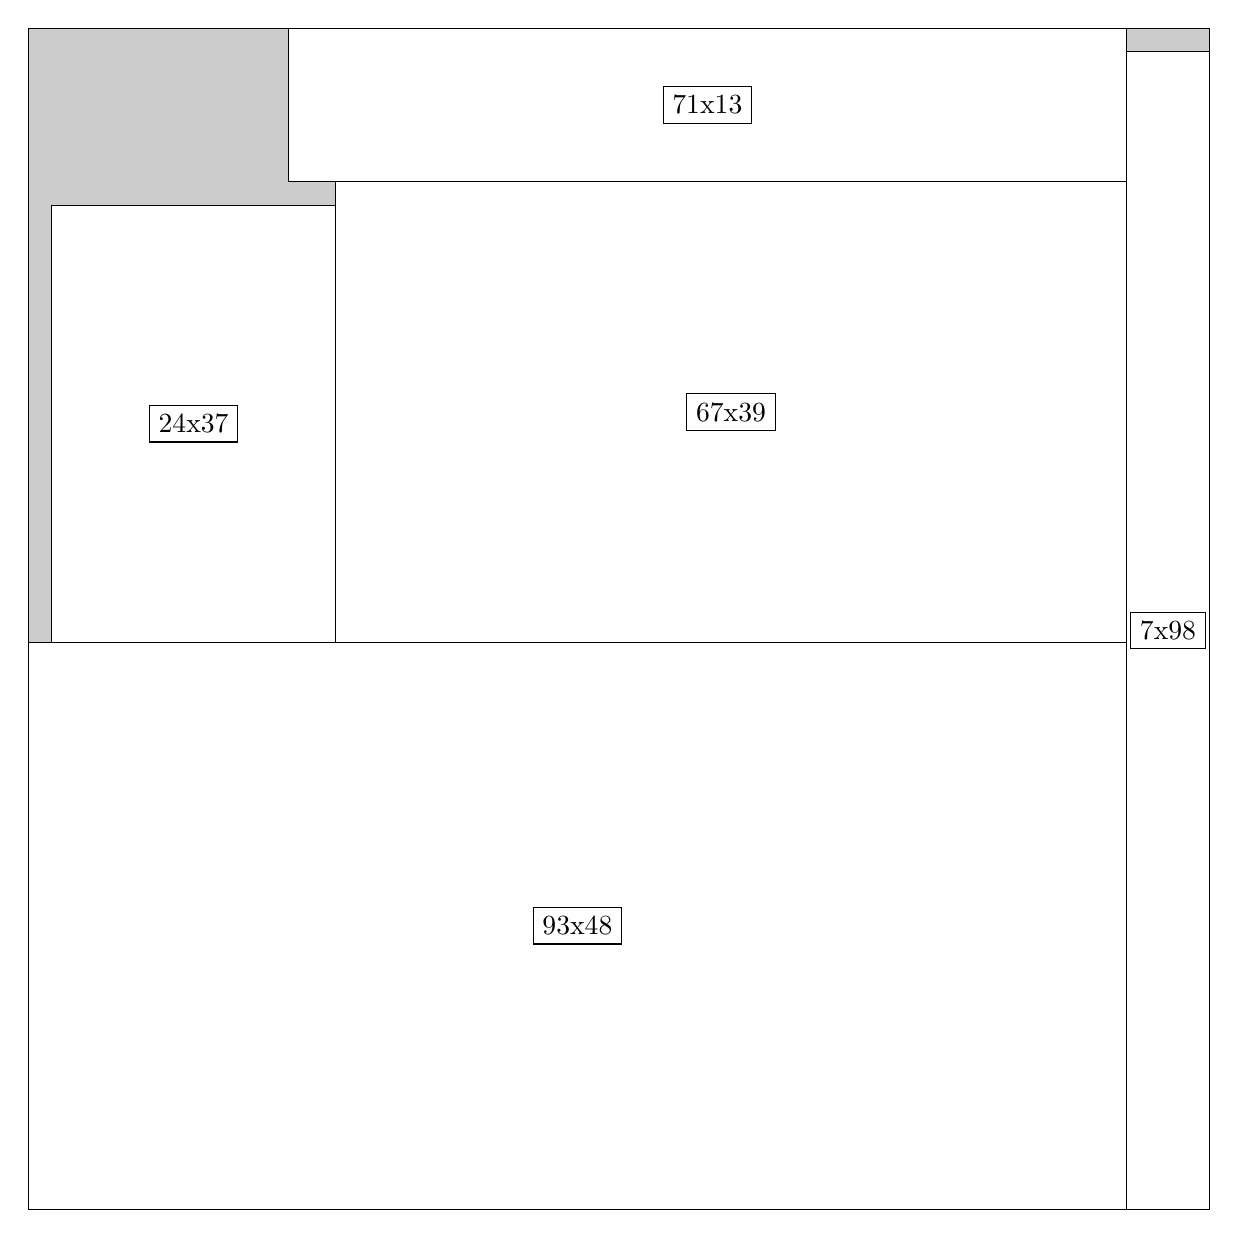
\begin{tikzpicture}[shorten >=1pt,scale=1.0,every node/.style={scale=1.0},->]
\tikzstyle{vertex}=[circle,fill=black!25,minimum size=14pt,inner sep=0pt]
\filldraw[fill=gray!40!white, draw=black] (0,0) rectangle (15.0,15.0);
\foreach \name/\x/\y/\w/\h in {7x98/13.95/0.0/1.05/14.7,93x48/0.0/0.0/13.95/7.199999999999999,67x39/3.9/7.199999999999999/10.049999999999999/5.85,24x37/0.3/7.199999999999999/3.5999999999999996/5.55,71x13/3.3/13.049999999999999/10.65/1.95}
\filldraw[fill=white!40!white, draw=black] (\x,\y) rectangle node[draw] (\name) {\name} ++(\w,\h);
\end{tikzpicture}


w =7 , h =98 , x =93 , y =0 , v =686
\par
w =93 , h =48 , x =0 , y =0 , v =4464
\par
w =67 , h =39 , x =26 , y =48 , v =2613
\par
w =24 , h =37 , x =2 , y =48 , v =888
\par
w =71 , h =13 , x =22 , y =87 , v =923
\par
\newpage


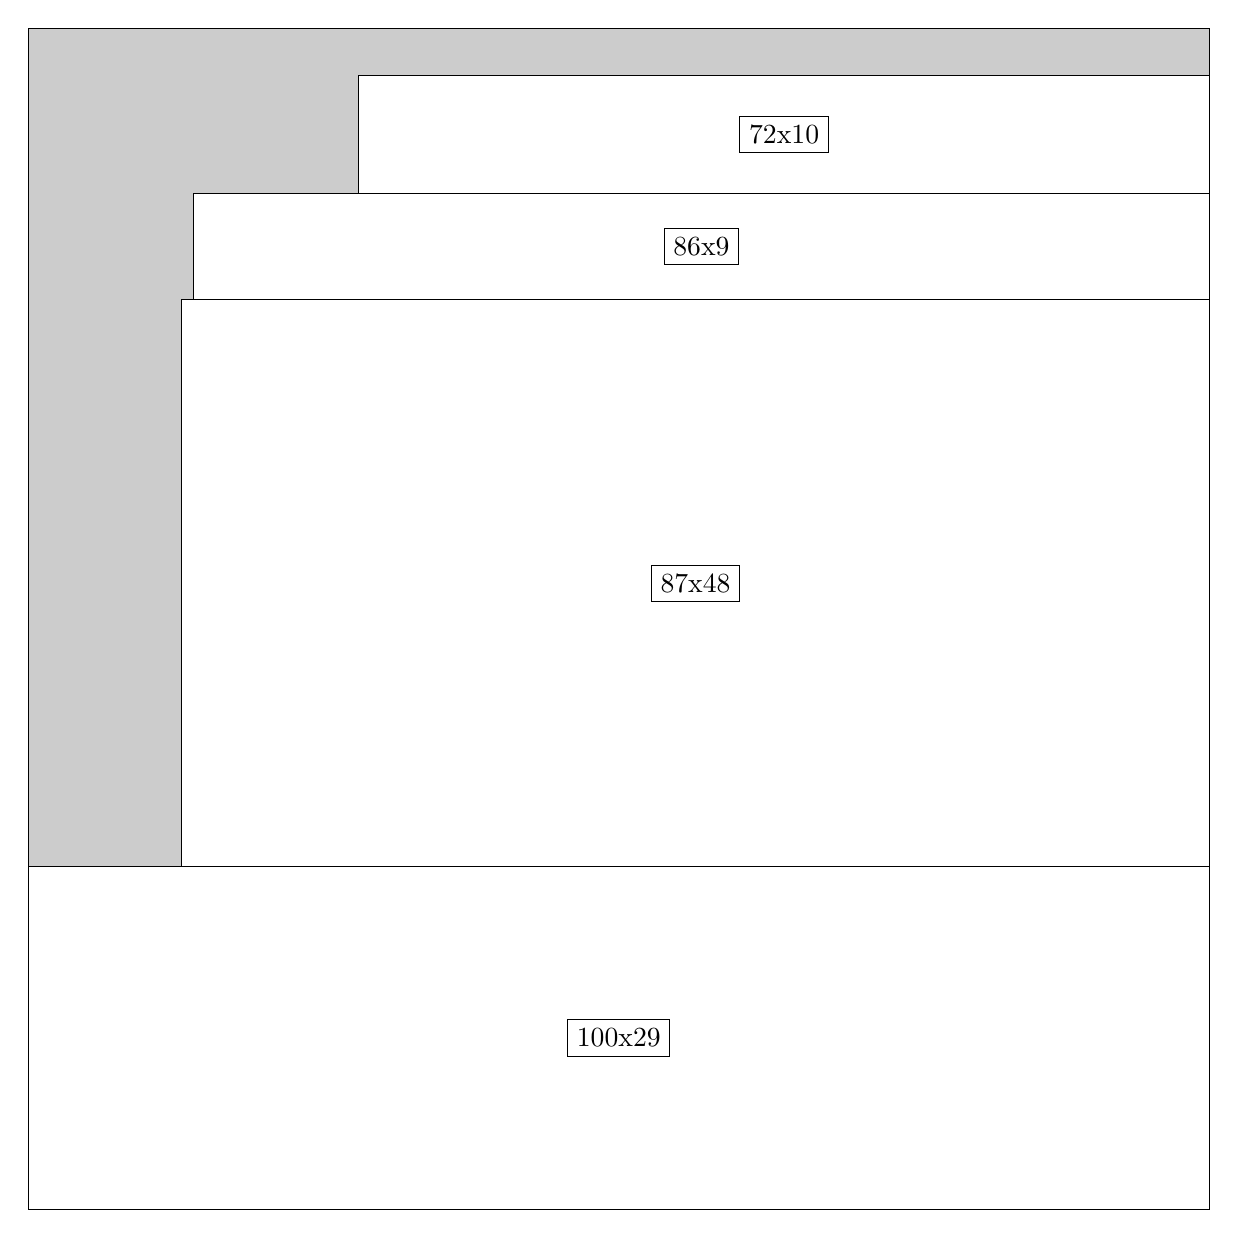
\begin{tikzpicture}[shorten >=1pt,scale=1.0,every node/.style={scale=1.0},->]
\tikzstyle{vertex}=[circle,fill=black!25,minimum size=14pt,inner sep=0pt]
\filldraw[fill=gray!40!white, draw=black] (0,0) rectangle (15.0,15.0);
\foreach \name/\x/\y/\w/\h in {100x29/0.0/0.0/15.0/4.35,87x48/1.95/4.35/13.049999999999999/7.199999999999999,86x9/2.1/11.549999999999999/12.9/1.3499999999999999,72x10/4.2/12.9/10.799999999999999/1.5}
\filldraw[fill=white!40!white, draw=black] (\x,\y) rectangle node[draw] (\name) {\name} ++(\w,\h);
\end{tikzpicture}


w =100 , h =29 , x =0 , y =0 , v =2900
\par
w =87 , h =48 , x =13 , y =29 , v =4176
\par
w =86 , h =9 , x =14 , y =77 , v =774
\par
w =72 , h =10 , x =28 , y =86 , v =720
\par
\newpage


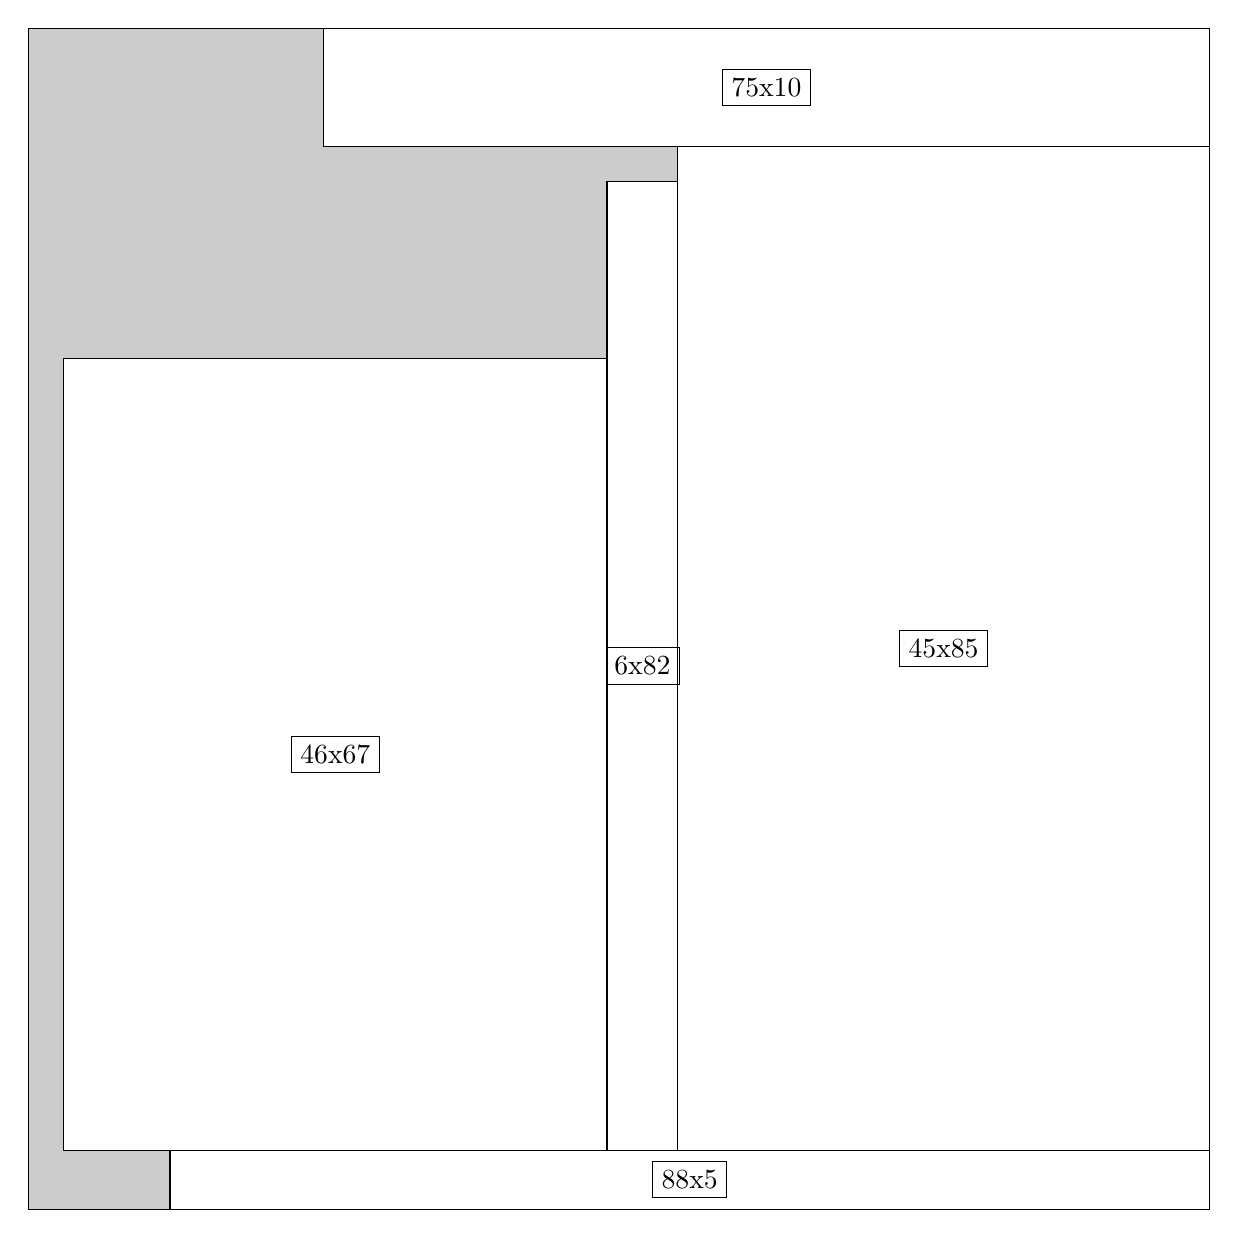
\begin{tikzpicture}[shorten >=1pt,scale=1.0,every node/.style={scale=1.0},->]
\tikzstyle{vertex}=[circle,fill=black!25,minimum size=14pt,inner sep=0pt]
\filldraw[fill=gray!40!white, draw=black] (0,0) rectangle (15.0,15.0);
\foreach \name/\x/\y/\w/\h in {88x5/1.7999999999999998/0.0/13.2/0.75,45x85/8.25/0.75/6.75/12.75,6x82/7.35/0.75/0.8999999999999999/12.299999999999999,46x67/0.44999999999999996/0.75/6.8999999999999995/10.049999999999999,75x10/3.75/13.5/11.25/1.5}
\filldraw[fill=white!40!white, draw=black] (\x,\y) rectangle node[draw] (\name) {\name} ++(\w,\h);
\end{tikzpicture}


w =88 , h =5 , x =12 , y =0 , v =440
\par
w =45 , h =85 , x =55 , y =5 , v =3825
\par
w =6 , h =82 , x =49 , y =5 , v =492
\par
w =46 , h =67 , x =3 , y =5 , v =3082
\par
w =75 , h =10 , x =25 , y =90 , v =750
\par
\newpage


\end{document}